%! TeX program = xelatex
\newcommand{\PFF}[1]{./body/aux/experiments/#1}
\documentclass[../ml-ct.tex]{subfiles}
\begin{document}
\chapter{Generative Regularizers for Computed Tomography Reconstruction}%
\label{chap:experiments}
\myepigraph{Radiologists who use AI will replace radiologists who don't.}{Curtis Langlotz}{RSNA 2017}

\minitoc%
In this chapter, we will detail our model as well as the specifics of the training procedure.
Subsequently, we will put our regularizer to test by considering typical reconstruction problems, such as limited-angle and few-view \gls{ct} reconstruction.
Additionally, we will exploit the generative properties of the regularizer.
Specifically, we can \emph{sample} the \emph{posterior distribution} for any given problem, and likewise visualize the associated \emph{prior} of our regularizer by drawing samples from it or exploring its modes.

\section{Model and Training}%
\label{sec:experiments}
We start by specifying our model architecture, which is based on~\cite{nijkamp_anatomy_2019} and follows a traditional encoder-scheme.
The model is schematically shown in in~\cref{fig:experiments:architecture}.
We reduce the spatial dimension of the feature space using strided convolutions, where we blur the kernels following~\cite{zhang_convolutional_2019} to avoid aliasing artifacts.
All convolutions with the exception of the final, linear layer are followed by the leaky rectified linear unit activation function, with a leak coefficient of \num{0.05}.
We use \( N_f = \num{48} \) features in the first layer, resulting in in a total of \num{12179905} parameters.

To train our model, we use the Low Dose CT Image and Projection data-set~\cite{moen_lowdose_2020}, which we subsampled to a spatial resolution of \( \num{128} \times \num{128} \).
We draw samples from our model using the \gls{ula} as described in~\cref{alg:learning:mala}, which is run for \( T = 500 \) steps.
We further follow the idea of persistent \gls{cd}~\cite{tieleman_persistent_2008}, where we use a replay buffer holding \( N_\text{RB} = 8000 \) past images with a reinitialization chance of \SI{1}{\percent}.
Upon reinitialization of any given sample in the replay buffer, there is an equal chance of reinitialization with uniform noise or any sample from the training data set.
We optimize the \gls{ml} objective~\cref{eq:learning:ml objective final} using the Adam~\cite{kingma_adam_2015} optimizer with a learning rate of \num{5e-4}, and set the first and second order momentum variables to \( \beta_1 = \num{0.9} \) and \( \beta_2 = \num{0.999} \) respectively.
To stabilize training, we convolve the data distribution with a Gaussian distribution of standard deviation \( \sigma_\text{data} = \num{1.5e-2} \).
The training is summarized in~\cref{alg:experiments:training}.
\begin{figure}
	\centering
	\includestandalone[width=\textwidth]{\PFF{network}}
	\caption[Network architecture for learning generative regularizers.]{%
		Our network follows a typical encoder-structure, where \( \{%
			\tikz\node [
				draw, fill=threebythree, single arrow,
				minimum height=5mm,
				inner sep=0.5mm,
				single arrow head extend=1mm, anchor=west
			] at (0, 0){};,%
			\tikz\node [
				draw, fill=normalanno, single arrow,
				minimum height=5mm,
				inner sep=0.5mm,
				single arrow head extend=1mm, anchor=west
			] at (0, 0){};,%
			\tikz\node [
				draw, single arrow,
				minimum height=5mm,
				inner sep=0.5mm,
				single arrow head extend=1mm, anchor=west
			] at (0, 0){};%
		\} \) denote \( \{%
			\operatorname{relu} \circ \operatorname{conv}_{3, 1},
			\operatorname{relu} \circ \operatorname{conv}_{4, 2},
			\operatorname{conv}_{4, 1}%
		\} \), with the subscript specifying the filter size and stride.
		In the annotations, the upper value shows the spatial resolution of the feature space, and the lower value indicates the number of features.
	}%
	\label{fig:experiments:architecture}
\end{figure}
\begin{algorithm}[t]
	\DontPrintSemicolon%
	\SetKwInOut{Input}{Input}
	\SetKwInOut{Output}{Output}
	\Input{data distribution \( \distr{f} \), data smoothing variance \( \sigma_\text{data}^2 \), buffer length \( N_\text{RB} \), reinitialization chance \( p_{\text{re}} \), Langevin steps \( T \), initial parameters \( \params \), training epochs \(N_e\), Langevin step size \( \epsilon \)}
	\Output{learned maximum-likelihood parameters \( \optimal{\params}{} \)}
	Initialize replay buffer \( \mathcal{B} \leftarrow \{ u_1,\dotsc,u_{N_\text{RB}} \} \), \( u_i \sim \mathcal{U}{[0, 1]}^{128\cdot128} \)\;
	\For{\( t = 1,\dotsc,N_e\)}{
		Draw \( f^+ \sim \distr{f}, f^0 \sim \mathcal{B} \)\;
		Smooth data samples with \( f^+ \leftarrow f^+ + \nu_\text{data}, \nu_\text{data} \sim \mathcal{N}(0, \sigma_{\text{data}}\Id{}) \)\;
		\( \mathcal{B} \leftarrow \mathcal{B} \setminus \{ f^0 \} \)\;
		Generate \( f^- \) with~\cref{alg:learning:mala} using \( f^0 \), \( \epsilon \), \( T \)\;
		\( \mathcal{B} \leftarrow \mathcal{B} \cup \begin{cases}
			\{ f^- \} & \text{if}\ r \sim \mathcal{U}[0, 1] > p_{\text{re}}\\
			\{ f^+ \}\ \text{if}\ \bar{r} \sim \mathcal{U}[0, 1] < 0.5\ \text{else}\ \{ u_i \} \sim \mathcal{U}{[0, 1]}^{128\cdot128} & \text{else}
		\end{cases} \)\;
		\( \delta_{\params} = \grad{\params} (R(f^+, \params) - R(f^-, \params)) \)\;
		\( \params \leftarrow \operatorname{Adam}(\delta_{\params}) \)\;
	}
	\( \optimal{\params}{} = \params \)
	\caption{Persistent \gls{cd} training of an energy based model.}%
	\label{alg:experiments:training}
\end{algorithm}

For any of the inference tasks we use accelerated proximal gradient descent, as summarized in~\cref{alg:experiments:inference}.
This algorithm makes use of the proximal operator \( \Func{\operatorname{prox}}{\set{F}}{\set{F}} \), which for a function \( \Func{\gamma}{\set{F}}{\R} \) and \( \tau \in \R^+ \) is defined as
\begin{equation}
	\operatorname{prox}_{\tau \gamma} (\hat{f}) = \argmin_{f \in \set{F}} \bigg\{ \tau\gamma(f) + \frac{1}{2} \norm{f - \hat{f}}_2^2 \bigg\}.
\end{equation}
We point out how we solve the operator for different tasks in their respective sections.
Unless stated otherwise, we always run~\cref{alg:experiments:inference} with \( \alpha = \num{1e-2} \) and \( N_i = \num{1e3} \).
\section{Examining the Regularizer}
Before applying our learned regularizer to inference tasks, it is interesting to assess it on a data- and forward model independent basis.
The generative \gls{ml} learning scheme allows us to interpret the learned regularizer directly as a probability density function on the space of images.
The probability density is the Gibbs-Boltzmann distribution of \( R \), which reads as
\begin{equation}
	\pdf{M}(f, \theta) = \frac{\exp(-R(f, \params))}{\int_{\set{F}} \exp(-R(\zeta, \params))\ \dd \zeta}.%
\end{equation}
Naturally, it is interesting to consider the modes of \( \pdf{M} \), which by the above equation are easily seen to coincide with the modes of \( R \).
We find \( f_{\text{mode}} = \argmin_f R(f, \params) \) using~\cref{alg:experiments:inference} with \( D(f, p) = 0 \) and \( f^0 \sim \mathcal{U}{[0, 1]}^{128\cdot128} \).
The proximal operator \( \operatorname{prox}_{\alpha D(\cdot, p)} \) reduces to the identity mapping.

We show examples of \( f_\text{mode} \) in~\cref{fig:experiments:modes}.
To emphasize that these images indeed minimize our learned regularizer, we show example trajectories during minimization along with the corresponding energy in~\cref{fig:experiments:trajectories}.
\begin{algorithm}[t]
	\DontPrintSemicolon%
	\SetKwInOut{Input}{Input}
	\SetKwInOut{Output}{Output}
	\SetKw{Break}{break}
	\Input{Initial step size \( \alpha \), data \( p \), initial guess \( f^0 \), parameters \( \params \), iterations \( N_i \)}
	\Output{\(\optimal{f}{} = \argmin_{f} \big\{ E(f, p, \params) = D(f, p) + R(f, \params) \big\}\)}
	\( f^1 = f^0 \)\;
	\For{\( t = 1,\dotsc,N_i \)}{
		\( \bar{f} = f^{t} + \frac{t}{t + 3} (f^{t} - f^{t - 1}) \)\;
		\( g = \grad{1} R(\bar{f}, \params) \)\;
		\While{\( R(\operatorname{prox}_{\alpha D(\cdot, p)}(\bar{f} - \alpha g), \params) > R(\bar{f}, \params) + g\tp (f^{t} - \bar{f}) + \frac{1}{2\alpha} \norm{(f^{t} - \bar{f})}_2^2 \)}{
			\( \alpha \leftarrow \frac{\alpha}{2} \)\;
		}
		\( f^{t + 1} = \operatorname{prox}_{\alpha D(\cdot, p)}(\bar{f} - \alpha g) \)\;\label{alg:experiments:inference:prox-update}
		\( \alpha \leftarrow 2\alpha \)\;
	}
	\( \optimal{f}{} = f^{N_i} \)
	\caption{%
		Accelerated Proximal Gradient Descent for minimizing an energy functional.
	}%
	\label{alg:experiments:inference}
\end{algorithm}
\begin{algorithm}[t]
	\DontPrintSemicolon%
	\SetKwInOut{Input}{Input}
	\SetKwInOut{Output}{Output}
	\SetKw{Break}{break}
	\Input{\( A \in \R^{M\times N} \), \( f \in \R^N \), \( p \in \R^M \), iterations \( T \in \mathbb{N}^+ \)}
	\Output{\(\optimal{f}{} = \argmin_{f} \norm{Af -p}_2^2 \)}
	\( r^0 = Af - p \)\;
	\( u = r^0 \)\;
	\For{\( t = 0,\dotsc,T-1 \)}{
		\( \alpha = \frac{{(r^t)}\tp r^t}{u\tp A u} \)\;
		\( f \leftarrow f + \alpha u \)\;
		\( r^{t + 1} = r^t - \alpha A u \)\;
		\( u \leftarrow r^{t + 1} + \frac{{(r^{t + 1})}\tp r^{t + 1}}{{(r^t)}\tp r^t} u \)\;
	}
	\( \optimal{f}{} = f \)
	\caption{%
		Conjugate Gradient Method to solve \( Af = p \).
	}%
	\label{alg:experiments:cg}
\end{algorithm}
\begin{figure}
	\centering
	\begin{tikzpicture}
		\foreach [count = \i] \num in {000, 001, 002, 003}
		{
			\node at (\i * 3.7, 0) {\includegraphics[width=3.5cm]{./aux/experiments/modes/nosampling_mode_\num.png}};
		}
		\foreach [count = \i] \num in {004, 005, 006, 007}
		{
			\node at (\i * 3.7, -4) {\includegraphics[width=3.5cm]{./aux/experiments/modes/nosampling_mode_\num.png}};
		}
	\end{tikzpicture}
	\caption[Examples of images which locally minimize the learned regularizer \( R \).]{%
		Examples of images which locally minimize the learned regularizer \( R \).
		The images were found using~\cref{alg:experiments:inference} with \( D(f, p) = 0 \) and initializing \( f^0 \) with uniform noise.
		We note that the samples closely resemble the training data, and want to emphasize that the model is able to learn small details in the images, such as blood vessels in the lung.
	}%
	\label{fig:experiments:modes}
\end{figure}
\begin{figure}
	\centering
	\scalebox{0.9}{\begin{tikzpicture}[trim axis left,trim axis right]
		\begin{axis}[
			height=3cm, width=17.58cm,
			restrict y to domain=-10:10, ymax=10,
			title={\( t \mapsto R(f^{t}, \phi) \)},
			grid=major,
			xmin=-50, xmax=950,
			xticklabels={},
			enlarge x limits=false, xtick={0,100,200,300,400,500,600,700,800, 900},
			title style={yshift=-1ex}
		]
			\addplot [domain=0:900,mark=none,photoncolor,thick] table [x=idx, y=c, col sep=comma] {./body/aux/experiments/mode_sampling/energies.csv};
		\end{axis}
		\begin{scope}[xshift=-.8cm, yshift=-5.8cm]
			\foreach [count = \i] \step in {000, 100, 200, 300, 400, 500, 600, 700, 800, 900}
			{
				\pgfmathsetmacro{\xx}{\i * 1.6}
				\draw (\xx, 6) -- ++(0, -6.9);
				\node at (\xx, -1.1) {\num{\step}};
				\foreach \imagenum in {0, 1, 2, 3}
				{
					\pgfmathsetmacro{\yy}{\imagenum * 1.6}
					\pgfmathsetmacro{\xx}{\i * 1.6}
					\node at (\xx, \yy) {\includegraphics[width=1.5cm]{./aux/experiments/mode_sampling/\imagenum/\step.png}};
				}
			}
		\end{scope}
\end{tikzpicture}}
	\caption[Trajectories during minization of \( R \), starting from uniform noise.]{%
		Trajectories of the images from uniform noise to \( \argmin_f R(f, \params) \) along with the corresponding \( R(f^{t}, \params) \) over the iterations in~\cref{alg:experiments:inference}.
	}%
	\label{fig:experiments:trajectories}
\end{figure}
It can be observed that the modes are faithful representations of the training data set.
We further want to emphasize that the regularizer is able to learn and retain small details, such as the blood vessels in the lung or the shape of the vertebrae.

The analysis above yields a valuable insight into the regularizer, however it misses a great advantage of the energy-based approach, which is the ability to \emph{sample} the learned prior (or posterior, see~\cref{sec:experiments:posterior-sampling}).
To visualize samples from our learned prior, we run the \gls{ula} variant of~\cref{alg:learning:mala}, where we again choose \( f^0 \) as uniform noise.
We show the results for \( t \in \{ \num{1000}, \num{2000}, \num{5000}, \num{20000}, \num{39900} \} \) in~\cref{fig:experiments:sampling}.
\begin{figure}
	\centering
	\begin{tikzpicture}
		\foreach \imagenum in {0, 1, 2, 3}
		{
			\foreach [count = \i] \step in {1000, 2000, 5000, 20000, 39900}
			{
				\pgfmathsetmacro{\yy}{\imagenum * 2.2}
				\pgfmathsetmacro{\xx}{\i * 2.2}
				\node at (\xx, \yy) {\includegraphics[width=2cm]{./aux/experiments/sampling/\imagenum/\step.png}};
				\ifthenelse{\imagenum=0}{
					\node at (\xx, -1.2) {\( t = \num{\step} \)};
				}{}
			}
		}
	\end{tikzpicture}
	\caption[Trajectories of the images during Langevin sampling at different time steps.]{%
		Trajectories of the images during Langevin sampling at different time steps.
		Notice that that high-level features change significantly even for \( t \gg \).
		In other words, our sampling procedure is able to traverse different modes of the learned prior.
	}%
	\label{fig:experiments:sampling}
\end{figure}
The samples exhibit significant change even for very large \( t \).
In other words, we are able to traverse modes of the learned prior with the sampling procedure.

In accordance with~\cite{nijkamp_anatomy_2019}, we find that there is some difference between the modes and samples from the learned prior.
However, the effect of learning an implicit sampler rather than a faithful density does not seem to be too apparent.
That is, the learned modes also largely resemble the training data set, although the samples are a more faithful representation visually.
\section{Image-Space Inference}
In the previous section, we analyzed the learned prior in a data-independent way by minimizing or sampling it.
Here, we want to shift our focus to inference tasks in a post-processing-like framework.
Specifically, we consider
\begin{equation}
	\optimal{f}{} = \argmin_{f \in \mathcal{F}} \tilde{D}(f, \tilde{f}) + R(f, \params)
\end{equation}
where \( \tilde{f} \in \mathcal{F} \) is a corrupted \gls{ct} image.
To be precise, we let \( \tilde{f} = \operatorname{corr}(f_\text{gt}) \), where \( \operatorname{corr} \) is an image-space corruption such as Gaussian noise or information loss, and \( f_\text{gt} \) is a fully sampled and uncorrupted \gls{ct} reconstruction.
The data fidelity term \( \Func{\tilde{D}}{\mathcal{F} \times \mathcal{F}}{\R^+} \) is chosen accordingly and does not consider any forward operator \( A \).

For additive white Gaussian noise, we have \( \tilde{f} = f_\text{gt} + \nu \), \( \nu \sim \mathcal{N}(0, \sigma \Id{}) \) and it is known that squared  \( \ell_2 \) data term \( \tilde{D}(f, \tilde{f}) = \frac{\tilde{\lambda}}{2} \norm{f - \tilde{f}}_2^2 \) is optimal.
The proximal map \( \operatorname{prox}_{\alpha \tilde{D}(\cdot, \tilde{f})} \) can easily be solved in closed form as
\begin{equation}
	\operatorname{prox}_{\alpha \tilde{D}(\cdot, \tilde{f})}(f) = \frac{f + \alpha\tilde{\lambda}\tilde{f}}{1 + \alpha\tilde{\lambda}}.
\end{equation}
We compare our method to the \gls{foe}~\cite{roth_fields_2005} and the \gls{tdv}~\cite{kobler_total_2020} models, as well as the \gls{tv} regularizer.
We find the optimal \( \tilde{\lambda} \) using a grid search approach.
We optimize the \gls{foe} model using~\cref{alg:experiments:inference}, and optimize the \gls{tv} model with a primal-dual algorithm~\cite{chambolle_primal_2010}.
The \gls{tdv} model is applied in an early stopping framework, as in the original work of~\cite{kobler_total_2020}.
We show quantitative \gls{psnr} values over an independent test set for \( \sigma \in \{ 15, 25, 50 \} \) in~\cref{tab:experiments:denoising}, along with visual examples in~\cref{fig:experiments:denoising}.
\begin{table}
	\centering
	\caption[Expected PSNR over the test set for denoising.]{%
		\( \mathbb{E}_{f\sim\distr{\bar{f}}}[\operatorname{PSNR}(\optimal{f}{}, f)] \) over a test distribution \( \distr{\bar{f}} \) for denoising.
	}%
	\label{tab:experiments:denoising}
	\begin{tabular}{S[table-format=2]*4S[table-format=2.2]}
		\toprule
		{\( \sigma \)} & {\gls{tv}} & {\gls{foe}} & {\gls{tdv}} & {Ours}  \\\toprule
		15 & 30.71    & 34.97     & 37.59     & 35.93 \\
		25 & 29.00    & 32.44     & 34.89     & 33.39 \\
		50 & 27.78    & 28.45     & 30.92     & 30.04 \\\bottomrule
	\end{tabular}
\end{table}
\begin{figure}
	\centering
	\scalebox{0.8}{
	\begin{tikzpicture}[spy using outlines={rectangle,lens={scale=3}, size=2cm, connect spies}]
		\def\imwidth{2}
		\def\ppad{0.2}

		\foreach [count = \imethod] \method in {\gls{tv}, \gls{foe}, \gls{tdv}, Ours}{
			\node at (1.1+\imethod *2* 2.2, 8) {\method};
		}
		\foreach [count = \imethod] \method in {tv, foe, tdv, ours}{
			\foreach [count = \isigma] \ssigma in {15, 25, 50}{
				\pgfmathsetmacro{\xx}{\imethod * 2 * (\imwidth + \ppad)}
				\pgfmathsetmacro{\yy}{\isigma * (\imwidth + \ppad)}
				\ifthenelse{\imethod=1}{
					\node [rotate=90] at (\xx - \imwidth + 0.6, \yy) {\( \sigma = \ssigma \)};
				}{}
				\node at (\xx, \yy) {\includegraphics[width=2cm]{./aux/experiments/denoise/\method/denoise\ssigma_\method_final.png}};
			}
		}
		\spy [blue] on (0 * 4.4 + 4.5, 2) in node [left] at (0 * 4.4 + 5.5+2,2.2);
		\spy [blue] on (1 * 4.4 + 4.5, 2) in node [left] at (1 * 4.4 + 5.5+2,2.2);
		\spy [blue] on (2 * 4.4 + 4.5, 2) in node [left] at (2 * 4.4 + 5.5+2,2.2);
		\spy [blue] on (3 * 4.4 + 4.5, 2) in node [left] at (3 * 4.4 + 5.5+2,2.2);

		\spy [blue] on (0 * 4.4 + 4.5, 4.2) in node [left] at (0 * 4.4 + 5.5+2,4.4);
		\spy [blue] on (1 * 4.4 + 4.5, 4.2) in node [left] at (1 * 4.4 + 5.5+2,4.4);
		\spy [blue] on (2 * 4.4 + 4.5, 4.2) in node [left] at (2 * 4.4 + 5.5+2,4.4);
		\spy [blue] on (3 * 4.4 + 4.5, 4.2) in node [left] at (3 * 4.4 + 5.5+2,4.4);

		\spy [blue] on (0 * 4.4 + 4.5, 6.4) in node [left] at (0 * 4.4 + 5.5+2,6.6);
		\spy [blue] on (1 * 4.4 + 4.5, 6.4) in node [left] at (1 * 4.4 + 5.5+2,6.6);
		\spy [blue] on (2 * 4.4 + 4.5, 6.4) in node [left] at (2 * 4.4 + 5.5+2,6.6);
		\spy [blue] on (3 * 4.4 + 4.5, 6.4) in node [left] at (3 * 4.4 + 5.5+2,6.6);
	\end{tikzpicture}}
	\caption[Results for a denoising task for \( \sigma \in \{ \num{15}, \num{25}, \num{50} \} \).]{%
		Results for a denoising task for \( \sigma \in \{ \num{15}, \num{25}, \num{50} \} \).
		Our approach retains significantly more detail, however it also hallucinates some structures into the image.
	}%
	\label{fig:experiments:denoising}
\end{figure}

Although the \gls{tdv} regularizer beats our approach in the quantitative \gls{psnr} analysis, we observe that our regularizer is able to retain much more details in the reconstruction.
A drawback of our approach is that for high noise levels, where we set \( \tilde{\lambda} \ll \) and as such allow the regularizers more freedom, it is able to hallucinate some structures into the image that do not appear in the ground truth reconstruction.
However, similar things can be said for the other approaches, which typically lose small structures in the image, due to their implicit or explicit preference for piecewise constant solutions.

As the next task, we consider image inpainting.
Here, we assume that we know a subset \( \mathcal{I} \) of the image domain \( \Omega \) exactly, whereas we have no information in \( \tilde{\mathcal{I}} = \Omega \setminus \mathcal{I} \).
From this, a natural choice for the data term is the Dirac distribution
\begin{equation}
	\tilde{D}(f, \tilde{f}) = \delta_{\mathcal{I}}(f, \tilde{f}) = \begin{cases}
		\infty & \text{if}\ f\neq \tilde{f}\ \text{anywhere in}\ \mathcal{I}, \\
		0 & \text{else},
	\end{cases}
\end{equation}
where the proximal operator decays to the projection
\begin{equation}
	\operatorname{prox}_{\alpha\delta_{\mathcal{I}}(\cdot, \tilde{f})} (f) =  \begin{cases}
		\tilde{f} &\ \text{in}\ \mathcal{I},\\
		f & \text{else}.
	\end{cases}
\end{equation}

Specifically, we will consider two cases that differ in the nature of \( \mathcal{I} \):
\begin{enumerate}
	\item Line inpainting: For each horizontal line in \( \Omega \), there is a chance \( p_i \) that its pixels are in \( \tilde{\mathcal{I}} \).
	\item Pixel inpainting: Each pixel in \( \Omega \) has a chance \( p_i \) to be in \( \mathcal{I} \).
\end{enumerate}

We show the \gls{psnr} values over an independent test set for \( p_i \in \{ 0.5, 0.8, 0.9 \} \) in~\cref{tab:experiments:inpainting}, and show qualitative results in~\cref{fig:experiments:inpainting}.
We want to bring attention to the fact that \gls{psnr} analysis becomes more and more meaningless as \( p_i \) increases, since there is more and more ambiguity and natural reconstructions may be far from the initial image.
\begin{table}
	\centering
	\caption[Expected PSNR over the test set for inpainting.]{
		\( \mathbb{E}_{f\sim\distr{\bar{f}}}[\operatorname{PSNR}(\optimal{f}{}, f)] \) over a test distribution \( \distr{\bar{f}} \) for different inpainting tasks.
	}%
	\label{tab:experiments:inpainting}
	\begin{tabular}{lS[table-format=1.1]*4S[table-format=2.2]}
		\toprule
		{Task} & {\( p_i \)} & {\gls{tv}} & {\gls{foe}} & {\gls{tdv}} & {Ours}  \\\toprule
		\multirow{3}{*}{Line} & 0.5 & 30.06    & 31.45     & 11.68     & 31.62 \\
				      & 0.8 & 23.58    & 24.20     & 9.82      & 23.70 \\
				      & 0.9 & 18.28    & 19.88     & 9.40      & 20.55 \\\midrule
		\multirow{3}{*}{Pixel}& 0.5 & 34.71    & 41.46     & 20.91     & 40.03 \\
				      & 0.8 & 29.59    & 33.02     & 15.22     & 33.44 \\
				      & 0.9 & 27.43    & 29.47     & 12.10     & 29.42 \\\bottomrule
	\end{tabular}
\end{table}
\begin{figure}
	\centering
	\scalebox{0.8}{
	\begin{tikzpicture}[spy using outlines={rectangle,lens={scale=3}, size=2cm, connect spies}]
		\def\imwidth{2}
		\def\ppad{0.2}
		\def\mode{px}
		\foreach [count = \imethod] \method in {\gls{tv}, \gls{foe}, \gls{tdv}, Ours}{
			\node at (1.1+\imethod *2* 2.2, 8) {\method};
		}
		
		\foreach [count = \imethod] \method in {tv, foe, tdv, ours}{
			\foreach [count = \isigma] \ppp in {0.50, 0.80, 0.90}{
				\pgfmathsetmacro{\xx}{\imethod * 2 * (\imwidth + \ppad)}
				\pgfmathsetmacro{\yy}{\isigma * (\imwidth + \ppad)}
				\node at (\xx, \yy) {\includegraphics[width=2cm]{./aux/experiments/inpaint/\method/inpaint\mode_\ppp_\method_final.png}};
			}
		}
		\foreach [count = \isigma] \ppp in {0.5, 0.8, 0.9}{
			\pgfmathsetmacro{\yy}{\isigma * (\imwidth + \ppad)}
			\node [rotate=90] at (3, \yy) {\( p_i = \num{\ppp} \)};
		}
		\spy [blue] on (0 * 4.4 + 4.5, 2) in node [left] at (0 * 4.4 + 5.5+2,2.2);
		\spy [blue] on (1 * 4.4 + 4.5, 2) in node [left] at (1 * 4.4 + 5.5+2,2.2);
		\spy [blue] on (2 * 4.4 + 4.5, 2) in node [left] at (2 * 4.4 + 5.5+2,2.2);
		\spy [blue] on (3 * 4.4 + 4.5, 2) in node [left] at (3 * 4.4 + 5.5+2,2.2);

		\spy [blue] on (0 * 4.4 + 4.5, 4.2) in node [left] at (0 * 4.4 + 5.5+2,4.4);
		\spy [blue] on (1 * 4.4 + 4.5, 4.2) in node [left] at (1 * 4.4 + 5.5+2,4.4);
		\spy [blue] on (2 * 4.4 + 4.5, 4.2) in node [left] at (2 * 4.4 + 5.5+2,4.4);
		\spy [blue] on (3 * 4.4 + 4.5, 4.2) in node [left] at (3 * 4.4 + 5.5+2,4.4);

		\spy [blue] on (0 * 4.4 + 4.5, 6.4) in node [left] at (0 * 4.4 + 5.5+2,6.6);
		\spy [blue] on (1 * 4.4 + 4.5, 6.4) in node [left] at (1 * 4.4 + 5.5+2,6.6);
		\spy [blue] on (2 * 4.4 + 4.5, 6.4) in node [left] at (2 * 4.4 + 5.5+2,6.6);
		\spy [blue] on (3 * 4.4 + 4.5, 6.4) in node [left] at (3 * 4.4 + 5.5+2,6.6);
	\begin{scope}[shift={(0, -7.5)}]
		\def\imwidth{2}
		\def\ppad{0.2}
		\def\mode{line}
		
		\foreach [count = \imethod] \method in {tv, foe, tdv, ours}{
			\foreach [count = \isigma] \ppp in {0.50, 0.80, 0.90}{
				\pgfmathsetmacro{\xx}{\imethod * 2 * (\imwidth + \ppad)}
				\pgfmathsetmacro{\yy}{\isigma * (\imwidth + \ppad)}
				\node at (\xx, \yy) {\includegraphics[width=2cm]{./aux/experiments/inpaint/\method/inpaint\mode_\ppp_\method_final.png}};
			}
		}
		\foreach [count = \isigma] \ppp in {0.5, 0.8, 0.9}{
			\pgfmathsetmacro{\yy}{\isigma * (\imwidth + \ppad)}
			\node [rotate=90] at (3, \yy) {\( p_i = \num{\ppp} \)};
		}
		\spy [blue] on (0 * 4.4 + 4.5, -7.5 + 2) in node [left] at (0 * 4.4 + 5.5+2,-7.5 + 2.2);
		\spy [blue] on (1 * 4.4 + 4.5, -7.5 + 2) in node [left] at (1 * 4.4 + 5.5+2,-7.5 + 2.2);
		\spy [blue] on (2 * 4.4 + 4.5, -7.5 + 2) in node [left] at (2 * 4.4 + 5.5+2,-7.5 + 2.2);
		\spy [blue] on (3 * 4.4 + 4.5, -7.5 + 2) in node [left] at (3 * 4.4 + 5.5+2,-7.5 + 2.2);

		\spy [blue] on (0 * 4.4 + 4.5, -7.5 + 4.2) in node [left] at (0 * 4.4 + 5.5+2,-7.5 + 4.4);
		\spy [blue] on (1 * 4.4 + 4.5, -7.5 + 4.2) in node [left] at (1 * 4.4 + 5.5+2,-7.5 + 4.4);
		\spy [blue] on (2 * 4.4 + 4.5, -7.5 + 4.2) in node [left] at (2 * 4.4 + 5.5+2,-7.5 + 4.4);
		\spy [blue] on (3 * 4.4 + 4.5, -7.5 + 4.2) in node [left] at (3 * 4.4 + 5.5+2,-7.5 + 4.4);

		\spy [blue] on (0 * 4.4 + 4.5, -7.5 + 6.4) in node [left] at (0 * 4.4 + 5.5+2,-7.5 + 6.6);
		\spy [blue] on (1 * 4.4 + 4.5, -7.5 + 6.4) in node [left] at (1 * 4.4 + 5.5+2,-7.5 + 6.6);
		\spy [blue] on (2 * 4.4 + 4.5, -7.5 + 6.4) in node [left] at (2 * 4.4 + 5.5+2,-7.5 + 6.6);
		\spy [blue] on (3 * 4.4 + 4.5, -7.5 + 6.4) in node [left] at (3 * 4.4 + 5.5+2,-7.5 + 6.6);
	\end{scope}
	\end{tikzpicture}}
	\caption[Results for an inpainting task for \( p_i \in \{ \num{0.5}, \num{0.8}, \num{0.9} \} \).]{%
		Results for an inpainting task for \( p_i \in \{ \num{0.5}, \num{0.8}, \num{0.9} \} \).
		The top three rows show a pixel-wise inpainting problem, and the bottom three rows depict a line-wise inpainting problem.
		We find that our approach leads to the most natural and detailed reconstructions visually.
	}%
	\label{fig:experiments:inpainting}
\end{figure}
We find that our approach leads to the most natural and detailed reconstructions, especially as the percentage of missing information increases, that is as \( p_i \rightarrow 1 \).
We attribute this to the fact that our regularizer has a global receptive field and as such can draw correspondences over large distances.
Further, we see that the \gls{tdv} regularizer, which was trained discriminatively on an additive Gaussian denoising tasks fails catastrophically at this task, as it tries to smooth image and hallucinates very unnatural structures into the image.
\section{Model-Based Reconstruction}
In this section, we will apply our learned prior to \gls{ct} reconstruction tasks.
Specifically, we will focus on limited-angle and few-view \gls{ct} reconstruction.
Recall that our forward model is given by
\begin{equation}
	p = Af + \nu,%
\end{equation}
and we are trying to find 
\begin{equation}
	\optimal{f}{} = \argmin_{f \in \set{F}}\ \bigl\{ E(f, p, \params) \coloneq D(f, p) + R(f, \params) \bigr\}.
\end{equation}
In what follows, we use the ASTRA toolbox~\cite{vanaarle_astra_2016,vanaarle_astra_2015} to discretize our forward operator \( A \) using the scheme detailed in~\cref{fig:image:discretized model}.
We also use their implementation of the traditional reconstruction algorithms, namely \gls{sart} and \gls{fbp}.
For all experiments, we let \( \nu \) be \( \SI{0.1}{\percent} \) Gaussian noise and use 
\begin{equation}
	D(f, p) = \frac{\lambda}{2} \norm{Af - p}_2^2,
\end{equation}
where we find \( \lambda \) using grid-search.
We run the \gls{sart} algorithm for \num{5000} iterations, and solve the \gls{tv} problem using \num{400} iterations of the primal-dual algorithm~\cite{chambolle_primal_2010}.
We solve the proximal maps with~\cref{alg:experiments:cg} using \( T = 10 \) iterations.

Recall that, for~\cref{alg:experiments:inference}, we need to compute
\begin{equation}
	\operatorname{prox}_{\alpha D(\cdot, p)} (\hat{f}) = \argmin_{f\in\set{F}} \bigg\{ \rho(f) \coloneq \frac{\alpha\lambda}{2} \norm{Af - p}_2^2 + \frac{1}{2} \norm{f - \hat{f}}_2^2 \bigg\}.
\end{equation}
By construction, we know that \( \argmin_f \rho(f) \in \set{F} \), such that by convexity of \( \rho \)
\begin{equation}
	\optimal{f}{prox} = \operatorname{prox}_{\alpha D(\cdot, p)} (\hat{f}) \Leftrightarrow \grad{1}\rho(\optimal{f}{prox}) = 0.%
	\label{eq:experiments:prox-optimality}
\end{equation}
The condition~\cref{eq:experiments:prox-optimality} can be rewritten as
\begin{equation}
	(\alpha\lambda \bar{A}A+\Id{N})\optimal{f}{prox} = \alpha\lambda \bar{A} p + \hat{f},
\end{equation}
where \( \bar{A} \) is the adjoint of \( A \).
This can be solved using \gls{cg} as described in~\cref{alg:experiments:cg}.

We first consider the problem of limited angle \gls{ct} reconstruction.
Here, the sinogram is acquired only over a range of angles, which typically is considerably smaller than \( \pi\,\mathrm{rad} \).
Specifically, we sample \num{270} projections uniformly spaced over \( [0, \frac{\pi}{2}] \), with \num{362} detectors using a detector spacing of \num{1}\,pixel.
With our images discretized on a \( \num{128} \times \num{128} \) pixel grid, this results in a forward operator \( A \in \R^{(362 \cdot 270) \times (168\cdot168)} \).
We compare our method to \gls{fbp}, \gls{sart} and \gls{tv} reconstruction quantitatively in~\cref{tab:experiments:limited-angle} and show some examples of the reconstruction in~\cref{fig:experiments:limited-angle}.
\begin{table}
	\centering
	\caption[Expected PSNR over the test set for 90-degree limited angle reconstruction.]{
		\( \mathbb{E}_{f\sim\distr{\bar{f}}}[\operatorname{PSNR}(\optimal{f}{}, f)] \) over a test distribution \( \distr{\bar{f}} \) for limited-angle (\( \theta \in [0, \frac{\pi}{2}] \)) reconstruction.
	}%
	\label{tab:experiments:limited-angle}
	\begin{tabular}{l*4S[table-format=2.2]}
		\toprule
		Method & {\gls{fbp}} & {\gls{sart}} & {\gls{tv}} & {Ours}  \\\toprule
		\( \mathbb{E}_{f \sim \distr{\bar{f}}}[\operatorname{PSNR}(\optimal{f}{}, f)] \) & 19.05    & 27.72     & 29.67     & 34.21 \\\bottomrule
	\end{tabular}
\end{table}
\begin{figure}
	\centering
	\scalebox{0.95}{
	\begin{tikzpicture}[spy using outlines={chamfered rectangle, magnification=3, width=3cm, height=2cm, connect spies}]
		\foreach [count = \i] \method/\anno in {fbp/{\gls{fbp}}, sart/{\gls{sart}}, tv/{\gls{tv}}, ours/{Ours}}
		{
			\pgfmathsetmacro{\xx}{\i * 3.1}
			\node at (\xx, 0) {\includegraphics[width=3cm]{./aux/experiments/limited-angle/limited-angle_\method_final.png}};
			\node at (\xx, 1.8) {\anno};
		}
		\node at (0, 1.8) {Reference};
		\node at (0, 0) {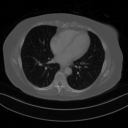
\includegraphics[width=3cm]{./aux/experiments/limited-angle/reference.png}};
		\spy [blue] on (0 * 3.1, -.4) in node [left] at (0 * 3.1 + 1.5, -2.2);
		\spy [blue] on (1 * 3.1, -.4) in node [left] at (1 * 3.1 + 1.5, -2.2);
		\spy [blue] on (2 * 3.1, -.4) in node [left] at (2 * 3.1 + 1.5, -2.2);
		\spy [blue] on (3 * 3.1, -.4) in node [left] at (3 * 3.1 + 1.5, -2.2);
		\spy [blue] on (4 * 3.1, -.4) in node [left] at (4 * 3.1 + 1.5, -2.2);
	\end{tikzpicture}}
	\caption[Qualitative results for limited-angle reconstruction.]{%
		Comparison between \gls{fbp}, \gls{sart}, \gls{tv}, and our method for limited-angle (\(\theta \in [0, \frac{\pi}{2}]\)) \gls{ct} reconstruction.
		Our model is able to faithfully reconstruct the image, whereas the other methods are not able to fully remove the limited-angle smearing artifacts.
	}%
	\label{fig:experiments:limited-angle}
\end{figure}

Our model is able to satisfactorily reconstruct the image, whilst the traditional unregularized reconstruction algorithms fail to faithfully restore the image.
This is especially apparent at contours where the projection streaks are not cancelled by other projections, such as in the upper left or lower right corners in~\cref{fig:experiments:limited-angle}.
Although \gls{tv} regularization helps alleviate this somewhat, the structures still look unnatural and it is not able to fully restore the contours.
On the other hand, the global receptive field of our approach allows to recover an image that is consistent with the training data.
Further, we want to point out that our model does not hallucinate any unwanted structures into the reconstruction, as the data term only allows changes to the image that are consistent with the measurement data.

An interesting avenue for dose reduction, which has come to light with the advent of \gls{cs}-based methods~\cite{donoho_compressed_2006}, is to perform angular undersampling~\cite{sidky_accurate_2006,sidky_reconstruction_2008}.
That is, as discussed in~\cref{sec:artifacts}, instead of densely sampling the Radon space in the rotational parameter we only acquire a few views, typically in the range of \num{100}.
For our experiments, we now sample \( N_\theta \) views uniformly spaced over \( [0, \pi] \), with \num{362} detectors each using a detector spacing of \num{1}\,pixel.
The expected \gls{psnr} values of our method along with traditional reference methods over a test set for \( N_\theta \in \{ 20, 30, 50, 100 \} \) are shown in~\cref{tab:experiments:undersampled}.
We further show a visual comparison in~\cref{fig:experiments:undersampled}.
\begin{table}
	\centering
	\caption[Expected PSNR over the test set for few-view CT reconstruction.]{%
		\( \mathbb{E}_{f \sim \distr{\bar{f}}} [\operatorname{PSNR}(\optimal{f}{}, f)]\) over a test distribution \( \distr{\bar{f}} \) for few-view \gls{ct} reconstruction using \( N_\theta \in \{ 20, 30, 50, 100 \} \).
	}%
	\label{tab:experiments:undersampled}
	\begin{tabular}{S[table-format=3]*4S[table-format=2.2]}
		\toprule
		{\( N_\theta \)} & {\gls{fbp}} & {\gls{sart}} & {\gls{tv}} & {Ours}  \\\midrule
		100 &  37.15   &   43.86   &   46.77   & 49.47 \\
		50 &  33.12    &   37.05   &   40.21   & 45.06 \\
		30 &  28.78    &   33.04   &   35.33   & 41.65 \\
		20 &  25.24    &   30.55   &   31.77   & 38.48 \\\bottomrule
	\end{tabular}
\end{table}
\begin{figure}
	\centering
	\scalebox{0.92}{
	\begin{tikzpicture}[spy using outlines={chamfered rectangle, magnification=3, width=3cm, height=2cm, connect spies}]
		\foreach [count = \imethod] \method/\anno in {fbp/{\gls{fbp}}, sart/{\gls{sart}}, tv/{\gls{tv}}, ours/{Ours}}
		{
			\foreach [count = \itheta] \ntheta in {50, 20}
			{
				\pgfmathsetmacro{\xx}{\imethod * 3.1}
				\pgfmathsetmacro{\yy}{-\itheta * 5.1}
				\node at (\xx, \yy) {\includegraphics[width=3cm]{./aux/experiments/undersampled/\ntheta/undersampled\ntheta_\method_final.png}};
				\ifthenelse{\itheta=1}{\node at (\xx, -5.1 + 1.8) {\anno}}{};
			}
		}
		\node [rotate=-90] at (14.2, -5.1) {\( N_\theta = 50 \)};
		\node [rotate=-90] at (14.2, -5.1 * 2) {\( N_\theta = 20 \)};
		\node at (0, -7.65 + 1.8) {Reference};
		\node at (0, -7.65) {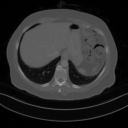
\includegraphics[width=3cm]{./aux/experiments/undersampled/reference.png}};
		\spy [blue] on (0 * 3.1, -7.65 -.4) in node [left] at (0 * 3.1 + 1.5, -7.65 -2.2);
		\spy [blue] on (1 * 3.1, -5.1 -.4) in node [left] at (1 * 3.1 + 1.5, -5.1 -2.2);
		\spy [blue] on (2 * 3.1, -5.1 -.4) in node [left] at (2 * 3.1 + 1.5, -5.1 -2.2);
		\spy [blue] on (3 * 3.1, -5.1 -.4) in node [left] at (3 * 3.1 + 1.5, -5.1 -2.2);
		\spy [blue] on (4 * 3.1, -5.1 -.4) in node [left] at (4 * 3.1 + 1.5, -5.1 -2.2);

		\spy [blue] on (1 * 3.1, -2*5.1 -.4) in node [left] at (1 * 3.1 + 1.5, -2*5.1 -2.2);
		\spy [blue] on (2 * 3.1, -2*5.1 -.4) in node [left] at (2 * 3.1 + 1.5, -2*5.1 -2.2);
		\spy [blue] on (3 * 3.1, -2*5.1 -.4) in node [left] at (3 * 3.1 + 1.5, -2*5.1 -2.2);
		\spy [blue] on (4 * 3.1, -2*5.1 -.4) in node [left] at (4 * 3.1 + 1.5, -2*5.1 -2.2);
	\end{tikzpicture}}
	\caption[Qualitative results for few-view CT reconstruction.]{%
		Comparison between \gls{fbp}, \gls{sart}, \gls{tv}, and our method for few-view \gls{ct} reconstruction.
		Our model is able to completely remove the streaking artifacts while retaining a satisfactory level of detail.
	}%
	\label{fig:experiments:undersampled}
\end{figure}

We again observe that our model is able to reconstruct the image satisfactorily, with small details such as the blood vessels in the lung visible even for \( N_\theta \) as low as \num{20}.
For such strong undersampling, we observe that \gls{fbp} reconstruction introduces very strong streaking artifacts, which are less apparent in the \gls{sart} reconstruction at the cost of an oversmoothed reconstruction.
\gls{tv} regularization is able to restore sharp edges from this, however we find that recovering a sharp images comes at the cost of losing almost all detail in the image, with only few gray levels remaining.
Our approach is able to eliminate the streaking artifacts whilst also retaining a good level of detail in the reconstruction.
The quantitative analysis in~\cref{tab:experiments:undersampled} also shows that our model outperforms the other reconstruction methods by a large margin.
\section{Posterior Sampling}%
\label{sec:experiments:posterior-sampling}
In the previous sections, we applied our learned prior to typical \gls{ct} reconstruction tasks.
There, we treated our regularizer as a point estimator, where the reconstruction is given as the \gls{map} of the Gibbs-Boltzmann distribution of the energy.
In other words, we computed
\begin{equation}
	\optimal{f}{MAP} = \argmin_{f \in \set{F}}\ \bigl\{ E(f, p, \params) \coloneq D(f, p) + R(f, \params) \bigr\}.
\end{equation}
However, our formulation allows us to leverage the full posterior distribution.
That is, we may also consider other estimators for the optimal solution, such as the expectation over the posterior
\begin{equation}
	\optimal{f}{E} = \mathbb{E}_{f \sim \distr{E}} [f] = \int_{\mathcal{F}} f \frac{\exp(-E(f, p, \params))}{\int_{\mathcal{F}} \exp(-E(\bar{f}, p, \params))\ \mathrm{d} \bar{f}}\ \mathrm{d}f,%
	\label{eq:experiments:expectation}
\end{equation}
where \( \distr{E} \) is the Gibbs-Boltzmann distribution of \( E(f, p, \params) \) given the parameters \( \params \).
Clearly, it is intractable to solve~\cref{eq:experiments:expectation} analytically, but we may approximate it using \gls{lmc}, or simply visually examine samples from the posterior.

To visualize this, we use the same few-view and limited-angle forward operator as in the previous section using \( N_\theta = \num{30} \) and \( \theta \in [0, \frac{\pi}{2}] \) respectively.
We inject noise into~\cref{alg:experiments:inference} after computing the proximal map in~\cref{alg:experiments:inference:prox-update}, where we draw the noise from \( \mathcal{N}(0, \alpha\beta \Id{}) \), where \( \beta \) is chosen as \( \beta = \num{2e-3} \).
We show a sampling trajectory along with the mean and variance over all iterations in~\cref{fig:experiments:posterior-sampling}.
We observe high variance around small structures such as the vertebrae and the blood vessels in the lung, and along contours for few-view reconstruction as well as regions of high ambiguity in the limited-angle reconstruction (c.f.~~\cref{fig:experiments:limited-angle}).
\begin{figure}
	\centering
	\scalebox{0.75}{\begin{tikzpicture}[spy using outlines={rectangle, lens={scale=3}, width=3cm, height=2cm, connect spies}]
		\def\imwidth{3}
		\def\ppad{0.1}
		\foreach [count = \timecount] \ttime in {50, 100, 150, 199} {
			\pgfmathsetmacro{\xx}{\timecount * (\imwidth + \ppad)}
			\node at (\xx, 0) {\includegraphics[width=\imwidth cm]{./aux/experiments/posterior_sampling/\ttime.png}};
		}
		\pgfmathsetmacro{\xxleft}{1 * (\imwidth + \ppad) - .2 - \imwidth/2}
		\pgfmathsetmacro{\xxright}{4 * (\imwidth + \ppad) + .2 + \imwidth/2}
		\draw (\xxleft, 1.2) -- ++(0, 0.4) -- node [midway, above] {\(f \sim \distr{E} \)} (\xxright, 1.6) -- ++(0, -0.4);
		\pgfmathsetmacro{\xx}{5 * (\imwidth + \ppad) + 0.3}
		\node at (\xx, 0) {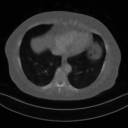
\includegraphics[width=\imwidth cm]{./aux/experiments/posterior_sampling/mean.png}};
		\node at (\xx, 1.8) {\( \mathbb{E}_{f\sim\distr{E}}[f] \)};
		\pgfmathsetmacro{\xx}{6 * (\imwidth + \ppad) + 0.3}
		\node at (\xx, 0) {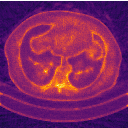
\includegraphics[width=\imwidth cm]{./aux/experiments/posterior_sampling/std.png}};
		\node at (\xx, 1.8) {\( \mathbb{V}_{f\sim\distr{E}}[f] \)};
		\spy [blue] on (1 * 3.1 + .1, -.4) in node [left] at (1 * 3.1 + 1.5, -2);
		\spy [blue] on (2 * 3.1 + .1, -.4) in node [left] at (2 * 3.1 + 1.5, -2);
		\spy [blue] on (3 * 3.1 + .1, -.4) in node [left] at (3 * 3.1 + 1.5, -2);
		\spy [blue] on (4 * 3.1 + .1, -.4) in node [left] at (4 * 3.1 + 1.5, -2);
		\spy [blue] on (5 * 3.1 + .1 + 0.3, -.4) in node [left] at (5 * 3.1 + 1.5 + 0.3, -2);
		\spy [blue] on (6 * 3.1 + .1 + 0.3, -.4) in node [left] at (6 * 3.1 + 1.5 + 0.3, -2);
	\begin{scope}[yshift=-5cm]
		\foreach [count = \timecount] \ttime in {50, 100, 150, 199} {
			\pgfmathsetmacro{\xx}{\timecount * (\imwidth + \ppad)}
			\node at (\xx, 0) {\includegraphics[width=\imwidth cm]{./aux/experiments/posterior_sampling/limited-angle/\ttime.png}};
		}
		\pgfmathsetmacro{\xxleft}{1 * (\imwidth + \ppad) - .2 - \imwidth/2}
		\pgfmathsetmacro{\xxright}{4 * (\imwidth + \ppad) + .2 + \imwidth/2}
		\pgfmathsetmacro{\xx}{5 * (\imwidth + \ppad) + 0.3}
		\node at (\xx, 0) {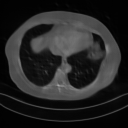
\includegraphics[width=\imwidth cm]{./aux/experiments/posterior_sampling/limited-angle/mean.png}};
		\pgfmathsetmacro{\xx}{6 * (\imwidth + \ppad) + 0.3}
		\node at (\xx, 0) {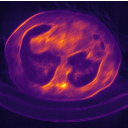
\includegraphics[width=\imwidth cm]{./aux/experiments/posterior_sampling/limited-angle/std.png}};
	\end{scope}
	\spy [blue] on (1 * 3.1 -0.5, -5+.5) in node [left] at (1 * 3.1 + 1.5, -5-2);
	\spy [blue] on (2 * 3.1 -0.5, -5+.5) in node [left] at (2 * 3.1 + 1.5, -5-2);
	\spy [blue] on (3 * 3.1 -0.5, -5+.5) in node [left] at (3 * 3.1 + 1.5, -5-2);
	\spy [blue] on (4 * 3.1 -0.5, -5+.5) in node [left] at (4 * 3.1 + 1.5, -5-2);
	\spy [blue] on (5 * 3.1 -0.5 + 0.3, -5+.5) in node [left] at (5 * 3.1 + 1.5 + 0.3, -5-2);
	\spy [blue] on (6 * 3.1 -0.5 + 0.3, -5+.5) in node [left] at (6 * 3.1 + 1.5 + 0.3, -5-2);
	\end{tikzpicture}}
	\caption[Samples, expected value and variance of the posterior of a few-view CT reconstruction problem.]{%
		Sampling the posterior of a few-view (\( N_\theta = 30 \), top) and limited-angle  (\( \theta \in [0, \frac{\pi}{2}]\), bottom) \gls{ct} reconstruction problem:
		The four images on the left show different samples during the sampling process, the two images on the right show the expected sample and variance of the posterior distribution respectively.
	}%
	\label{fig:experiments:posterior-sampling}
\end{figure}
\section{A Note on Scale-Non-Invariance and Out-Of-Distribution Application}
In the architecture of our regularizer, we explicitly consider the image size, as the repeated strided convolutions directly map from \( \num{128} \times \num{128} \) to a scalar.
This means that our network is explicitly not invariant with respect to the scale of the image, or in other words, we have learned a prior on \gls{ct} images of exactly this resolution.  However, since the network is composed only of convolutional layers (as opposed to fully connected layers), we may apply it to different resolution images.
\begin{figure}
	\centering
	\begin{tikzpicture}
		\def\imwidth{3}
		\def\ppad{0.1}
		\foreach [count = \iscale] \scale in {256, 512} {
			\foreach [count = \isigma] \ssigma in {25, 50} {
				\pgfmathsetmacro{\xx}{\iscale * (\imwidth + \ppad)}
				\pgfmathsetmacro{\yy}{\isigma * (\imwidth + \ppad)}
				\node at (\xx, \yy) {\includegraphics[width=\imwidth cm]{./aux/experiments/scales/scale_\ssigma_\scale.png}};
				\ifthenelse{\isigma=1}{
					\node at (\xx, 8) {\( \num{\scale} \times \num{\scale} \)};
				}{}
				\ifthenelse{\iscale=1}{
					\node [rotate=90] at (1.2, \yy) {\(\sigma = \ssigma\)};
				}{}
			}
		}
		\pgfmathsetmacro{\xx}{4 * (\imwidth + \ppad) + 0.5}
		\pgfmathsetmacro{\yy}{1.5 * (\imwidth + \ppad)}
		\node at (\xx, \yy) {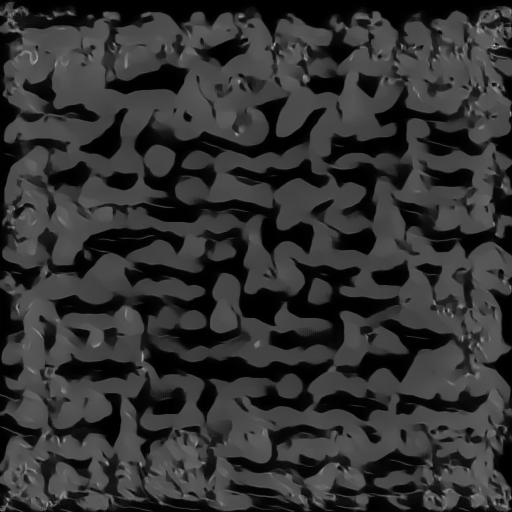
\includegraphics[width=\imwidth cm]{./aux/experiments/scales/scale_512_sample.png}};
		\node at (\xx, \yy + 1.8) {Sample};
		\pgfmathsetmacro{\xx}{3 * (\imwidth + \ppad) + 0.1}
		\pgfmathsetmacro{\yy}{1.5 * (\imwidth + \ppad)}
		\node at (\xx, \yy) {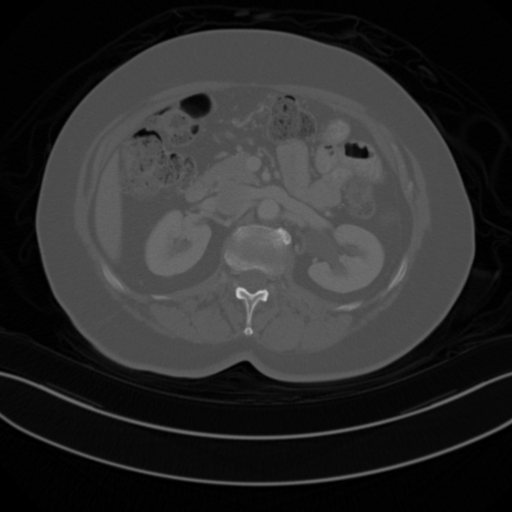
\includegraphics[width=\imwidth cm]{./aux/experiments/scales/reference.png}};
		\node at (\xx, \yy + 1.8) {Reference};
	\end{tikzpicture}
	\caption[Demonstration of scale-non-invariance of our regularizer.]{%
		Experiments on different scales:
		Results for Gaussian denoising and a sample of our prior on \( \num{512} \times \num{512} \).
		Since our regularizer is not scale-invariant, the results are not satisfactory.
	}%
	\label{fig:experiments:scale-denoising}
\end{figure}

To examine the behavior in such cases, we consider an image-space denoising task for different resolutions \( \num{256} \times \num{256} \) and \( \num{512} \times \num{512} \).
We solve the denoising problem using accelerated proximal gradient descent for \( \sigma \in \{ 25, 50 \} \), and show the results along with a sample of our model on these resolutions in~\cref{fig:experiments:scale-denoising}.
We see that, even for a denoising task with \( \sigma = \num{25} \), the regularizer is not able to restore the image satisfactorily, as it hallucinates new structures into the image while the noise is is still apparent.
In general, due to the design of our regularizer, we can not expect it to work on resolutions other than the training resolution.

To study the behavior on out-of-distribution samples, we perform the following denoising experiment:
We let
\begin{equation}
	f_{\kappa} = \operatorname{rot}_{\kappa} (f) + \nu,
\end{equation}
where \( \Func{\operatorname{rot}_\kappa}{\mathcal{F}}{\mathcal{F}} \) is the bilinear rotation operator of angle \( \kappa \) and \( \nu \sim \mathcal{N}(0, \sigma\Id{}) \), \( \sigma = \num{25} \).
We determine the optimal \( \tilde{\lambda} \) using manual grid search on \( f_{0} \), and show expected \gls{psnr} values in~\cref{fig:experiments:ood-plot} for \( \kappa \in \{ \SI{1}{\degree}, \SI{2}{\degree}, \SI{3}{\degree}, \SI{4}{\degree}, \SI{5}{\degree}, \SI{10}{\degree},\dotsc, \SI{40}{\degree} \} \).
\begin{figure}
	\centering
	\begin{tikzpicture} [>=latex]
		\begin{axis}[
			ymin=27,
			ymax=34,
			grid=major,
			width=\textwidth,
			height=4cm,
			title={\( \kappa \mapsto \mathbb{E}_{f \sim \distr{\bar{f}}} [\operatorname{PSNR}(\optimal{f}{}, \operatorname{rot}_\kappa (f))] \)},
			name=plot,
			title style={yshift=-1ex},
		]
			\addplot [photoncolor, mark=x] table [x=x,y=y] {
				x    y
				0    33.39
				1    32.62
				2    31.81
				3    31.43
				4    30.73
				5    30.25
				10   29.62
				15   28.50
				20   28.33
				25   28.17
				30   28.09
				35   28.35
				40   28.20
			};
			\node (kappa0) [draw, rectangle, light] at (axis cs:0,33.39) {};
			\node (kappa5) [draw, rectangle, light] at (axis cs:5,30.25) {};
			\node (kappa40) [draw, rectangle, light] at (axis cs:40,28.20) {};
		\end{axis}
		\begin{scope}[xshift=1.5cm, yshift=-2.7cm]
			\foreach \offset/\kkappa in {0/0, 5/5, 10/40}
			{
				\node at (\offset, 0) {\includegraphics[width=4cm]{./aux/experiments/ood/denoise_rot_\kkappa_ours_final.png}};
				\node (\kkappa) [light, draw, rectangle, minimum width=4.2cm, minimum height=4.2cm] at (\offset, 0) {};
				\draw [light] (kappa\kkappa.south) -- (\kkappa.north);
			}
		\end{scope}
	\end{tikzpicture}
	\caption[Denoising results for out-of-distribution data.]{%
		Performance of the regularizer on out-of-distribution data:
		For denoising rotated images, the \gls{psnr} quickly decays even for small rotations.
	}%
	\label{fig:experiments:ood-plot}
\end{figure}
We can see that the \gls{psnr} value quickly decreases even for small \( \kappa \).
For larger \( \kappa \), the model introduces unnatural structures in the image visually, which goes hand in hand with a strong drop in quantitative performance.
In general, since our model is a strong prior only for \enquote{upright} \gls{ct} images, performance quickly degrades even for small affine transformations on the images drawn from the training distribution.
\end{document}
